\usepackage[utf8]{inputenc}
\bibliographystyle{apalike}
\usepackage{bibentry}
\nobibliography*
\usepackage{slovak}
\usepackage{tikz}
\usetikzlibrary{arrows,positioning}
\usetheme{Warsaw}
\title{Biologicky motivované \\výpočtové modely}
\author{Michal Kováč}
\institute{FMFI UK}
\date{24.6.2013}
\begin{document}
\renewcommand{\pause}{}

\begin{frame}[t]
\titlepage
\end{frame}
\note{Vážená komisia, \dots, chcel by som vám prezentovať moje pokroky v dizertačnej práci.}

\section*{Outline}
\begin{frame}
\tableofcontents
\end{frame}
\note{
  Prezentáciu začnem prehľadom existujúcich modelov, ktoré sú inšpirované biológiou.
  Potom budem hovoriť o P systémoch, pretože im som sa najviac venoval.
  Existuje množstvo variantov, o ktorých niečo poviem v ďalšej časti.
  Prezentáciu zavŕšim predostretím plánov na dizertačnú prácu.
}

\section{Prehľad problematiky} % (fold)
\label{sec:prehlad_problematiky}

\subsection{Prehľad modelov} % (fold)
\label{sub:prehlad_modelov}

\begin{frame}[t]\frametitle{Biologicky motivované \\výpočtové modely}
  Dvojaké uplatnenie:
  \begin{itemize}
    \item reálne modely živých systémov
    \begin{itemize}
      \item virtuálne biologické experimenty
      \item verifikácia správnosti chápania ich činností
    \end{itemize}
    \item modely na popis iných systémov
  \end{itemize}
\end{frame}
\note{
  Biologicky motivované výpočtové modely majú dvojaké uplatnenie.

  Jednak v rámci biológie môžu slúžiť ako reálne modely správania sa živých systémov, na ktorých môžeme robiť rôzne virtuálne biologické experimenty, prípadne verifikovať správnosť nášho chápania ich biologickej činnosti.

  Na druhej strane môžu slúžiť ako modely na popis aj iných ako biologických systémov, čo otvára rad teoretických informatických otázok (napr. výpočtová sila)
}

\begin{frame}[t]\frametitle{Biologicky motivované \\výpočtové modely}
  \begin{itemize}
    \item Neurónové siete (od 1943)
    \item Celulárne automaty (od 1948)
    \item Evolučné algoritmy (od 1954)
    \item L systémy (od 1968)
    \item P systémy (od 1998) \cite{Paun98}
    \item Calculi of Looping Sequences (od 2007)
    \item Reaction systems (od 2007)
    \item \dots
  \end{itemize}
\end{frame}
\note{
  Dlho skúmané modely ako neurónové siete, celulárne automaty, evolučné algoritmy, či L systémy, si už našli svoje uplatnenie v praxi, kým membránové systémy sú ešte len v začiatkoch svojho vývoja.
}

% subsection prehlad_modelov (end)

\subsection{P systémy} % (fold)
\label{sub:p_systemy}

\begin{frame}[t]\frametitle{Membránová štruktúra}
  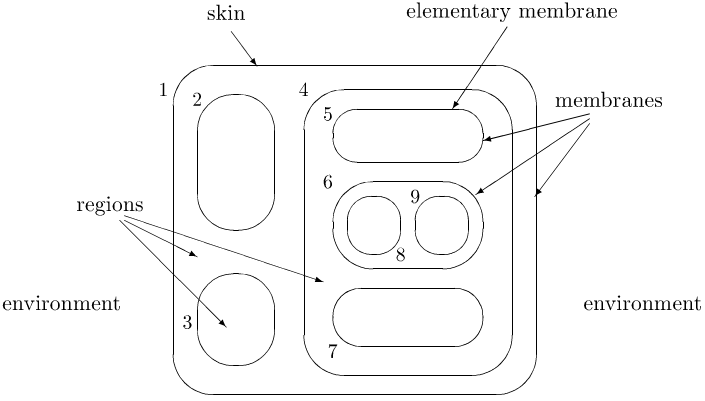
\includegraphics[width=0.7\textwidth]{membrane_structure.png}
  \hfill
  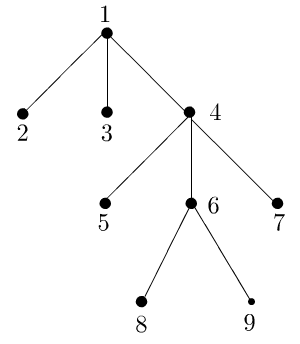
\includegraphics[width=0.3\textwidth]{membrane_tree.png}
  \pause
  \begin{itemize}
    \item Multisets
    \pause
    \item Rewriting rules
    \pause
    \item Passive vs. Active
  \end{itemize}

\end{frame}
\note{
  Membránové systémy sú inšpirované bunkami. Základom je preto membránová štruktúra, ktorá pozostáva z regiónov, ktoré sú oddelené membránami. Tvorí to hierarchickú štruktúru, ktorá sa dá zobraziť ako strom.
}

\begin{frame}[t]\frametitle{Varianty pravidiel}
  \begin{itemize}
    \item kooperatívne ($a\ |\ b\ |\ b \rightarrow b$) (RE \cite{Paun98})
    \pause
    \item nekooperatívne ($b \rightarrow c$) (CF \cite{Sburlan05dragos})
    \pause
    \item nekooperatívne s inhibítormi ($a \rightarrow b\ |_{\neg{c,d}}$) (ET0L \cite{Ionescu:jucs_10_5:on_p_systems_with})
    \pause
    \item katalytické ($a\ |\ b \rightarrow a\ |\ c\ |\ d$)
    \begin{itemize}
      \item katalytické s 2 katalyzátormi (RE \cite{Freund2005TwoCatalysts})
      \item s 1 katalyzátorom (otvorený problém)
      \item s 1 katalyzátorom a inhibítormi (RE \cite{Ionescu:jucs_10_5:on_p_systems_with})
    \end{itemize}
  \end{itemize}
\end{frame}
\note{}
\newpage
\note{}

\begin{frame}[t]\frametitle{Sekvenčné P systémy}
  \begin{itemize}
    \item Maximálny paralelizmus vs. sekvenčný mód
    \pause
    \item Sekvenčné P systémy s kooperatívnymi pravidlami (VASS \cite{Dang:2005:Sequential})
    \pause
    \begin{itemize}
      \item s prioritami (RE \cite{Dang:2005:Sequential})
      \pause
      \item s aktívnymi membránami (RE \cite{Dang:2005:Sequential})
      \pause
      \item {\bf s inhibítormi (RE \cite{Kovac14})}
    \end{itemize}
    \pause
    \item Jazyk
    \begin{itemize}
      \item Generatívny mód: postupnosť objektov vypustených do okolitého prostredia
      \pause
      \item Akceptačný mód: daná konfigurácia je akceptovaná, ak sa systém vie dostať do stavu, kde sa už nedá použiť žiadne pravidlo
    \end{itemize}
  \end{itemize}
\end{frame}
\note{}

% subsection p_systemy (end)

% section prehlad_problematiky (end)

\section{Skúmané varianty P systémov} % (fold)
\label{sec:sk_man_varianty_p_syst_mov}

\subsection{Sekvenčné P systémy s inhibítormi} % (fold)
\label{sub:sekven_n_p_syst_my_s_inhib_tormi}

\begin{frame}[t]\frametitle{Sekvenčné P systémy s inhibítormi}
  \begin{itemize}
    \item \bibentry{Kovac14}
  \end{itemize}
\end{frame}


\begin{frame}[t]\frametitle{Prehľad simulácie pre akceptačný mód}
  \begin{itemize}
    \item Simulácia registrového stroja
    \item Obsah registra $j$ sa reprezentuje početnosťou objektu $j$
    \item Objekt pre každú inštrukciu
    \pause
    \item SUB inštrukcia sa simuluje pomocou inhibítora
    \begin{itemize}
      \item $i: SUB(j,k,l)$
      \item $ij\rightarrow k$
      \item $i\rightarrow l|_{\neg{j}}$
    \end{itemize}
  \end{itemize}
\end{frame}
\note{}

\begin{frame}[t]\frametitle{Prehľad simulácie pre generatívny mód}
  \begin{itemize}
    \item Simulácia maximálne paralelného P systému $\Pi_1$ pomocou sekvenčného P systému s inhibítormi $\Pi_2$.
    \pause
    \item Každý maximálne paralelný krok $\Pi_1$ simulujeme sekvenčnými krokmi $\Pi_2$.
    \pause
    \item Produkty si označujeme, aby neboli použíté, kým neskončí daný maximálne paralelný krok.
    \pause
    \item Pomocou inhibítorov zistíme moment, kedy sa už v $\Pi_2$ nedá aplikovať žiadne pravidlo, aby sa mohol simulovať ďalší maximálne paralelný krok.
    \pause
    \item Synchronizácia medzi membránami pomocou tokenu.
  \end{itemize}
\end{frame}
\note{}

% subsection sekven_n_p_syst_my_s_inhib_tormi (end)

\subsection{Sekvenčné P systémy s aktívnymi membránami} % (fold)
\label{sub:sekven_n_p_syst_my_s_akt_vnymi_membr_nami}

\begin{frame}[t]\frametitle{Sekvenčné P systémy s aktívnymi membránami}
  \begin{itemize}
    \item Bez limitu počtu aplikovaní pravidla na vytvorenie membrány (RE \cite{Ibarra05Active})
    \pause
    \item \bibentry{Kovac15Active}
  \end{itemize}

  
\end{frame}

\begin{frame}[t]\frametitle{Problém zastavenia}
  \begin{itemize}
    \item Problém zastavenia je definovaný pre deterministické modely
    \pause
    \item Zovšeobecnenie: Existencia (ne)konečného výpočtu
  \end{itemize}

\end{frame}
\note{}

\begin{frame}[t]\frametitle{Existencia nekonečného výpočtu}
  \begin{itemize}
    \item Graf dosiahnuteľnosti
    \pause
    \item Čiastočné usporiadanie $\leq$:
    \begin{itemize}
      \item $C_1 \leq C_2 \Rightarrow$ každé pravidlo v $C_1$ je aplikovateľné v $C_2$.
      \pause
      \item Pre každú nekonečnú postupnosť konfigurácií existuje $C_1, C_2$: $C_1 \rightarrow^* C_2$ a $C_1 \leq C_2$.
    \end{itemize}
    \pause
    \item Dicksonova lemma: Pre každú nekonečnú postupnosť n-tíc nad $\mathbb{N}$ $\{a_i\}_{i=0}^\infty$ existujú $i<j$: $a_i\leq a_j$
  \end{itemize}
\end{frame}

\begin{frame}[t]{Algoritmus rozhodujúci existenciu nekonečného výpočtu}
  \begin{itemize}
    \item Traverzuj graf dosiahnuteľnosti
    \item Dosiahnutá konfigurácia $C_2$, taká, že na ceste z počiatočnej konfigurácie existuje $C_1\leq C_2\Rightarrow$ YES.
    \item Ak traverzovanie skončilo $\Rightarrow$ NO.
  \end{itemize}
\end{frame}

\begin{frame}[t]{Existencia konečného výpočtu}
  \begin{itemize}
    \item Pre daný P systém $\Pi$ a danú konfiguráciu $C$ vieme zostrojiť P systém $\Pi^\prime: \exists$ konečný výpočet $\Pi^\prime\Leftrightarrow C$ je dosiahnuteľná v $\Pi$.  
  \end{itemize}  
\end{frame}

% subsection sekven_n_p_syst_my_s_akt_vnymi_membr_nami (end)

\subsection{Detekcia prázdnosti membrán} % (fold)
\label{sub:detekcia_pr_zdnosti_membr_n}

\begin{frame}[t]{Detekcia prázdnosti membrán}
  \begin{itemize}
    \item Objekty vyhýbajúce sa prázdnym membránam
    \pause
    \item Mutovanie objektov pri poslaní do prázdnej membrány
    \pause
    \item Objekt reprezetujúci vákuum
  \end{itemize}  
\end{frame}

% subsection detekcia_pr_zdnosti_membr_n (end)

\subsection{Sekvenčné P systémy s množinami namiesto multimnožín} % (fold)
\label{sub:sekven_n_p_syst_my_s_mno_inami_namiesto_multimno_n}

\begin{frame}[t]{Sekvenčné P systémy s množinami namiesto multimnožín}
  \begin{itemize}
    \item \bibentry{Kovac15Set}
  \end{itemize}
\end{frame}

\begin{frame}[t]{Nevýhody používania multimnožín}
  \begin{itemize}
    \item Nakoľko realistické je reprezentovať presný počet objektov?
    \item Efektivita verifikačných techník
  \end{itemize}
\end{frame}

\begin{frame}[t]\frametitle{P systémy s množinami objektov}
  \begin{itemize}
    \item Alhazov \cite{Alhazov05WithoutMultiplicities}: počty objektov sa ignorujú (R), s aktívnymi membránami (RE)
    \item Kleijn, Koutny \cite{Kleijn11SetMembrane}: ``min-enabled'' computational step $\Rightarrow$ (R)
    \pause
    \item Maximálny paralelizmus $\Rightarrow$ determinizmus
    \pause
    \item Pravidlá bez konfliktu (objekty sa môžu zúčastniť ako reaktanty súčasne vo viacerých pravidlách)
  \end{itemize}
\end{frame}
\note{}

\begin{frame}[t]\frametitle{Sekvenčné P systémy s množinami objektov a aktívnymi membránami}
  \begin{itemize}
    \item $\Pi = (\Sigma, C_0, R_1, \ldots R_m)$
    \pause
    \item $C = (T, l, c)$
    \begin{itemize}
      \item $l: V(T) \rightarrow \{1, \ldots, m\}$
      \item $c: V(T) \rightarrow 2^\Sigma$
    \end{itemize}
    \pause
    \item Pravidlá
    \begin{itemize}
      \item $u\rightarrow w$
      \item $u\rightarrow w\delta$
      \item $u\rightarrow [_j v_1]_j v_2$,

      kde $u \in \Sigma, |u|\geq 1$, $v_1,v_2\in \mathbb{N}$ a $w\in (\Sigma\times\{\cdot, \uparrow, \downarrow_{j}\})$
    \end{itemize}

  \end{itemize}
\end{frame}
\note{}

\begin{frame}[t]\frametitle{Iné sémantiky vytvárania membrány}
  \begin{itemize}
    \item Problémy pôvodnej sémantiky:
    \begin{itemize}
      \item Vytváranie membrány, ktorá už existuje
      \item Posielanie objektu do neexistujúcej membrány
    \end{itemize}
    \pause
    \item Inject-or-create
    \pause
    \item Wrap-or-create
  \end{itemize}
\end{frame}

\begin{frame}[t]\frametitle{Simulácia registrového stroja}
  \begin{center}
    \begin{tabular}{c|c|c}
      \hline
      & priestor & čas \\ \hline
      original & $O(n)$ & $O(n)$ \\ \hline
      \pause
      original & $O(log(n))$ & $O(log(n))$ \\ \hline
      \pause
      inject-or-create & $O(log(n))$ & $O(log(n))$ \\ \hline
      \pause
      wrap-or-create & $O(n)$ & $O(1)$ \\ \hline
    \end{tabular}
  \end{center}
\end{frame}

% subsection sekven_n_p_syst_my_s_mno_inami_namiesto_multimno_n (end)

% section sk_man_varianty_p_syst_mov (end)


\begin{frame}[plain]
\begin{center}
  Ďakujem za pozornosť
\end{center}
\end{frame}

\begin{frame}[t]{Vyjadrenia k posudkom}
  \begin{itemize}
    \item Štandardnou motiváciou pre skúmanie týchto modelov je potenciál vysokého paralelizmu. Práca je príliš zameraná na sekvenčný mód, ktorý úplne eliminuje potenciál tohto modelu.
    \pause
    \item 
  \end{itemize}
\end{frame}

\newsavebox\mytempbib
\savebox\mytempbib{\parbox{\textwidth}{\bibliography{obhajoba}}}

\end{document}